\documentclass[11pt]{article}
\usepackage[a4paper,margin=2cm]{geometry}
\usepackage{graphicx,booktabs,amsmath,float,caption}
\usepackage[hidelinks]{hyperref}
\setlength{\parskip}{4pt}\setlength{\parindent}{0pt}

\title{\textbf{PRML Lab 10 --- Spam Classification with Support Vector Machines}}
\author{Aryan Tiwari (B20AI056)\\CSL2050 Pattern Recognition \& Machine Learning, Winter 2022}
\date{}

\begin{document}
\maketitle

\section{Methodology}

\textbf{Data.} UCI Spambase: 4{,}601 emails, 39.4\% spam, 57 numeric features --- 48 word frequencies, 6 character frequencies
(\texttt{!}, \texttt{\$}, \texttt{(} \dots) and 3 statistics of runs of capital letters. There are no missing values. The 391 repeated feature
vectors are kept, because the task asks for a random split of the data as given. The data was split at random into \textbf{70\% training
(3{,}220) and 30\% test (1{,}381)} emails, stratified so that both parts have the same spam share.

\textbf{Pre-processing.} The features are on very different scales (frequencies around 0--1, but \texttt{capital\_run\_length\_longest} has a
median of 15 and a maximum of 9{,}989). An SVM's margin and its polynomial/RBF kernels are built from inner products and distances, so every feature was
\textbf{standardised} with the training-set mean and standard deviation. The scaler sits inside a pipeline, so the test set never influences it.

\textbf{SVM package.} \texttt{sklearn.svm.SVC} (scikit-learn 1.6), which wraps \textbf{LIBSVM}. It solves the C-SVM dual problem
\[
\max_\alpha \sum_i\alpha_i - \tfrac12\sum_{i,j}\alpha_i\alpha_j y_i y_j K(x_i,x_j)\quad\text{s.t. } 0\le\alpha_i\le C,\ \textstyle\sum_i\alpha_i y_i=0
\]
with an SMO-type decomposition method. Kernels:
\begin{itemize}\itemsep0pt
\item \textbf{Linear:} $K(x,z)=x^\top z$
\item \textbf{Quadratic:} $K(x,z)=(\gamma\,x^\top z+1)^2$ (polynomial, degree 2, \texttt{coef0}=1, so that the linear and pairwise-interaction terms are both included)
\item \textbf{RBF:} $K(x,z)=\exp(-\gamma\lVert x-z\rVert^2)$
\end{itemize}
$\gamma$ is sklearn's \texttt{'scale'} default, $1/(d\cdot\mathrm{Var}(X)) = 1/57$ after standardisation. The generalisation constant
was tried at $C\in\{10^{-3},10^{-2},\dots,10^{3}\}$ for every kernel. The solver had no iteration limit: with a cap of $2\times10^5$
iterations the linear kernel stopped early at $C\ge100$ and its accuracy appeared to collapse to 61--78\%, which was an artefact of
the unfinished optimisation rather than a property of the model.

\begin{figure}[H]\centering
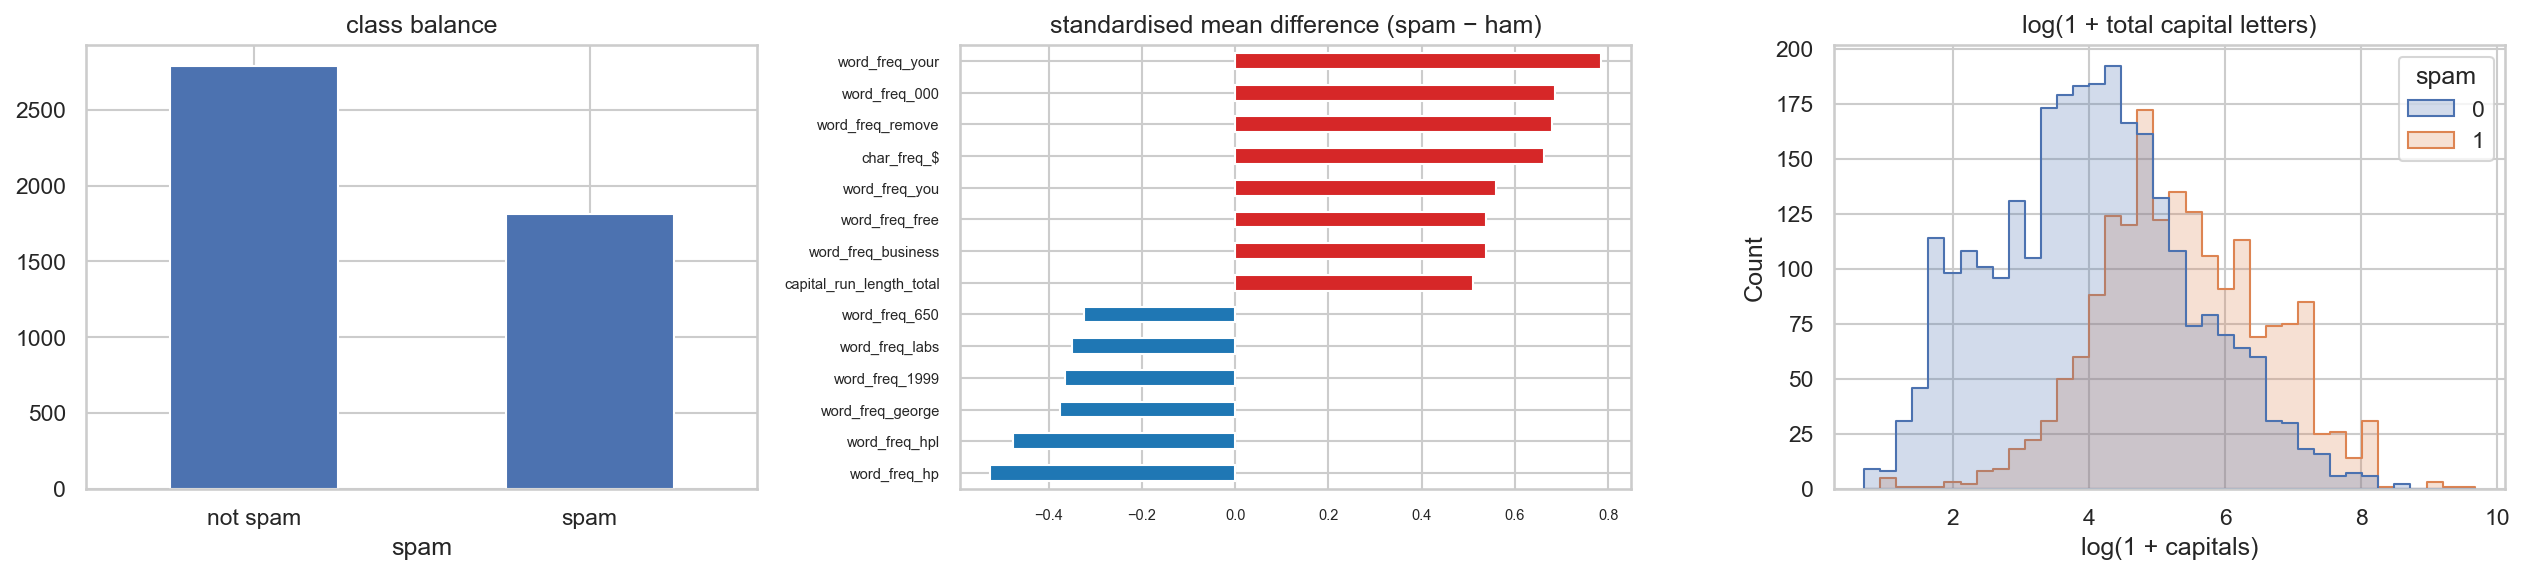
\includegraphics[width=\linewidth]{figures/eda.png}
\caption{Class balance; the features that differ most between spam and ham (standardised mean difference); total number of capital letters.}
\end{figure}

\section{Experimental results}

\subsection*{Accuracy for every value of C}
\begin{table}[H]\centering
\begin{tabular}{r|ccc|ccc}\toprule
 & \multicolumn{3}{c|}{Training accuracy} & \multicolumn{3}{c}{Test accuracy}\\
$C$ & Linear & Quadratic & RBF & Linear & Quadratic & RBF\\\midrule
0.001 & 0.8870 & 0.6115 & 0.6059 & 0.8892 & 0.6119 & 0.6061\\
0.01 & 0.9171 & 0.8460 & 0.7016 & 0.9218 & 0.8465 & 0.7009\\
0.1 & 0.9335 & 0.9199 & 0.9102 & 0.9341 & 0.9218 & 0.9088\\
1 & 0.9342 & 0.9447 & 0.9450 & 0.9305 & \textbf{0.9392} & 0.9341\\
10 & 0.9354 & 0.9590 & 0.9649 & 0.9341 & 0.9370 & \textbf{0.9392}\\
100 & 0.9354 & 0.9767 & 0.9845 & \textbf{0.9356} & 0.9327 & 0.9218\\
1000 & 0.9342 & 0.9891 & 0.9929 & 0.9348 & 0.9175 & 0.9117\\\bottomrule
\end{tabular}
\end{table}

\begin{figure}[H]\centering
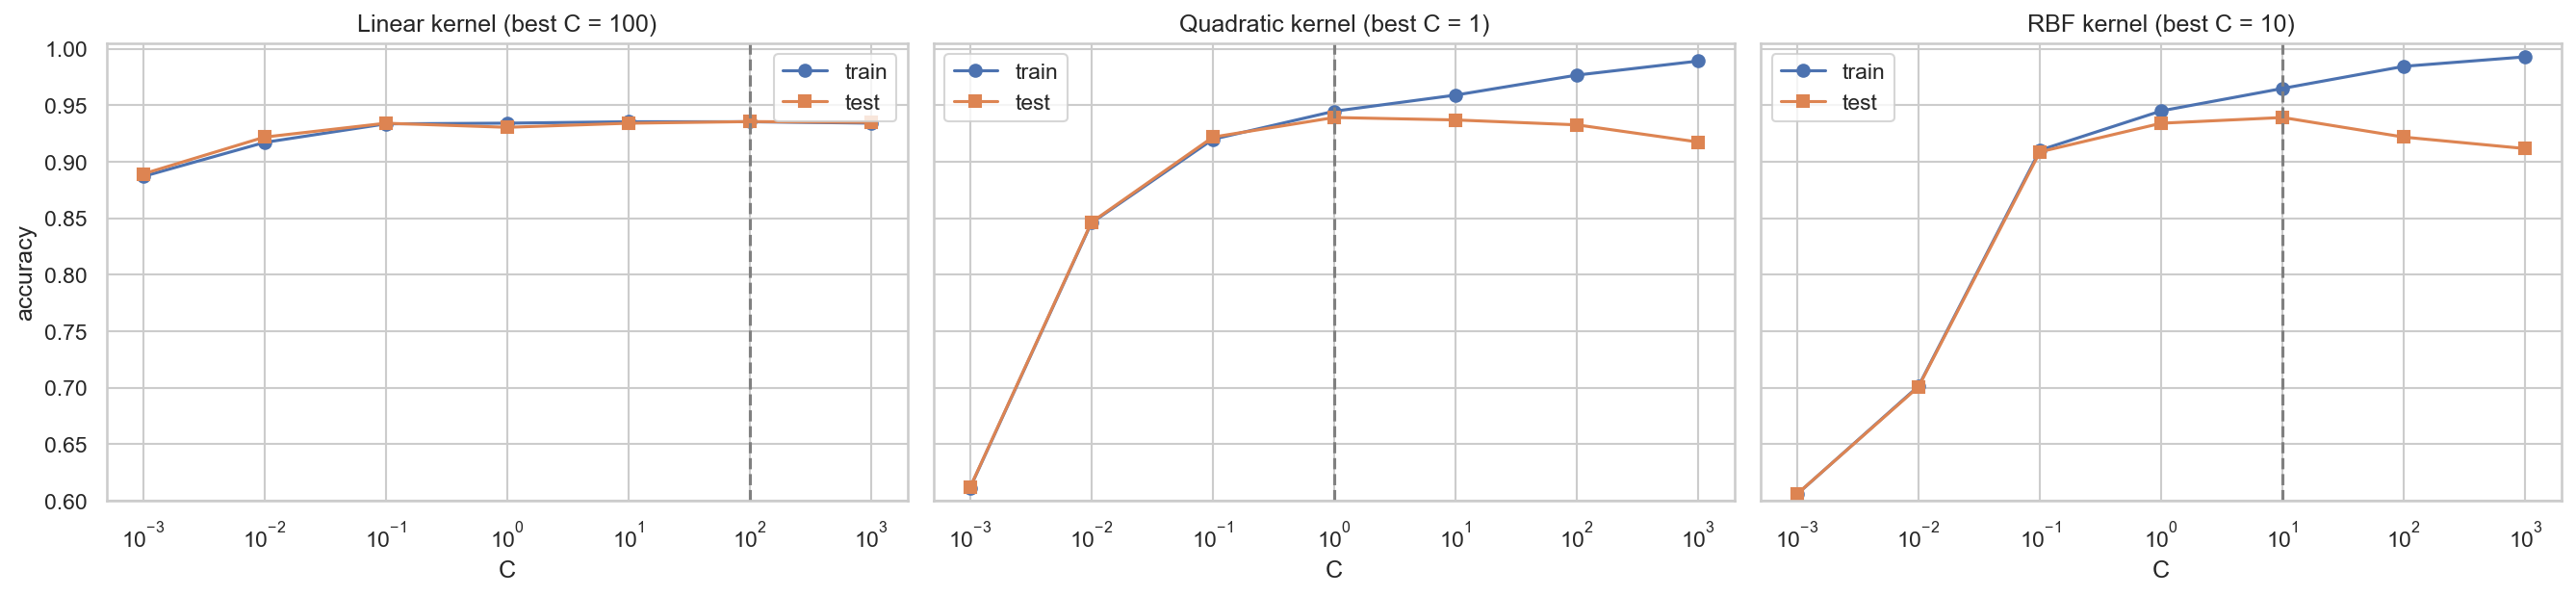
\includegraphics[width=\linewidth]{figures/accuracy_vs_C.png}
\caption{Training and test accuracy as a function of $C$ (dashed line: best $C$).}
\end{figure}

\subsection*{Comparison table --- best $C$ per kernel}
Following the assignment, the best $C$ is the one with the highest test accuracy:
\begin{table}[H]\centering
\begin{tabular}{lcccc}\toprule
Kernel & Best $C$ & Training accuracy & Test accuracy & Support vectors\\\midrule
Linear & 100 & 0.9354 & 0.9356 & 630\\
Quadratic & 1 & 0.9447 & \textbf{0.9392} & 767\\
RBF & 10 & 0.9649 & \textbf{0.9392} & 804\\\bottomrule
\end{tabular}
\end{table}

\textbf{Check on model selection.} Choosing $C$ by test accuracy uses the test set for model selection, so it slightly flatters the
result. As a check, I also chose $C$ by 5-fold cross-validation on the training set only. CV picks the same $C$ for the quadratic (1) and RBF (10)
kernels and $C=100$ for the linear kernel, so the reported test accuracies are \emph{unchanged}, and the comparison above is not
an artefact of tuning on the test set.

At their best $C$ the three kernels finish within 0.4 points of each other (93.6--93.9\%). On 1{,}381 test emails that is about 5 emails,
which is within noise. The spam class is detected with precision 0.93--0.94 and recall 0.90--0.91 for every kernel: roughly 35 legitimate
emails are flagged as spam and 50 spam emails get through.

\begin{figure}[H]\centering
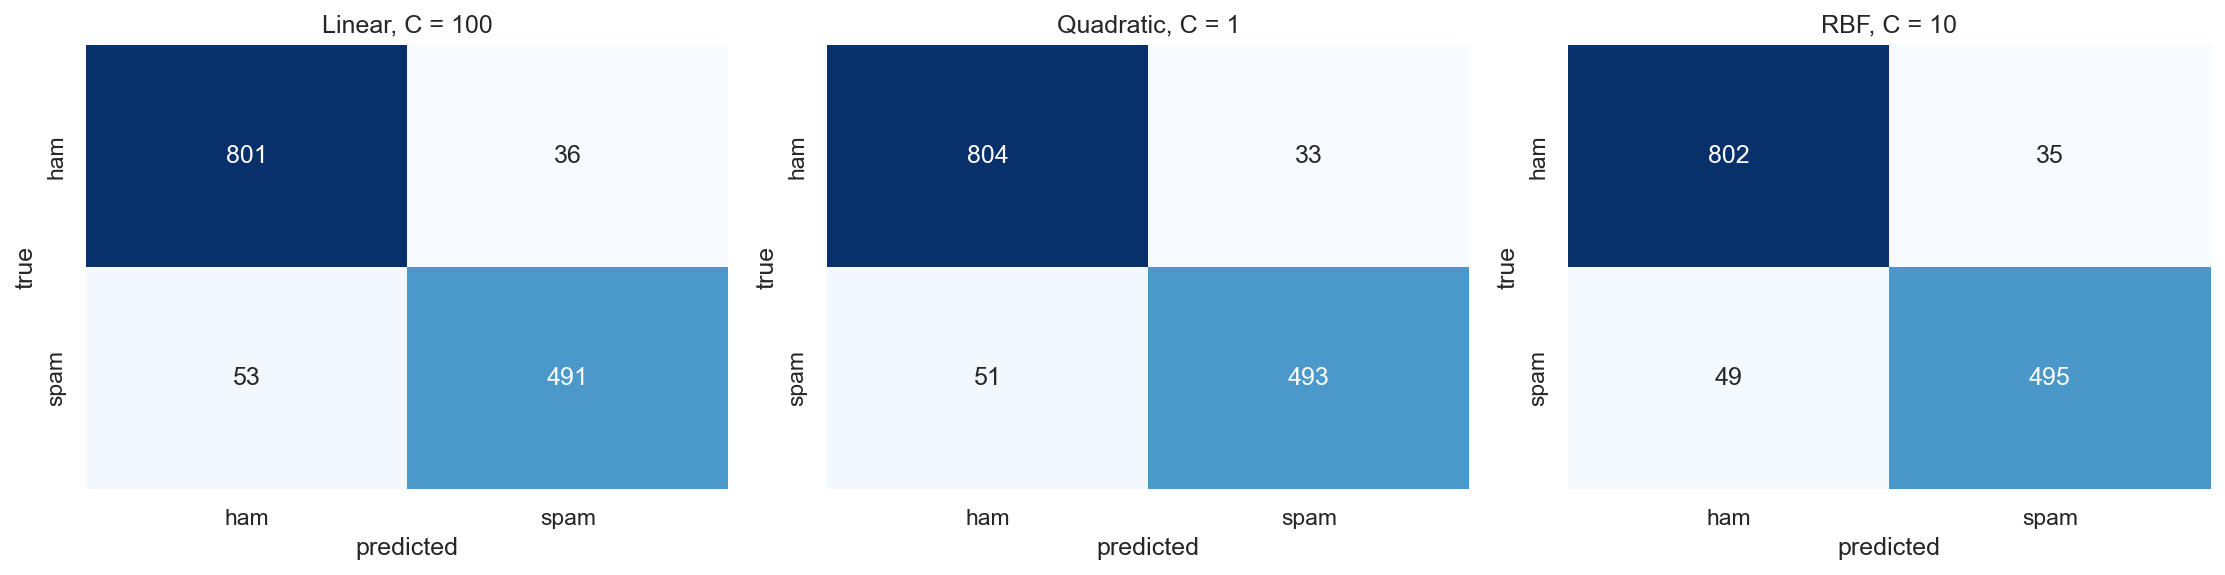
\includegraphics[width=0.85\linewidth]{figures/confusion.png}
\caption{Test-set confusion matrices at the best $C$ for each kernel.}
\end{figure}

\subsection*{Effect of $C$}
\begin{itemize}\itemsep0pt
\item \textbf{Small $C$} (wide, soft margin) \emph{underfits}. At $C=10^{-3}$ the quadratic and RBF machines barely beat always predicting ``not spam'' (61\%):
nearly every training point is a support vector (about 2{,}540 of 3{,}220), so the decision function is an almost flat average. The linear kernel
does better here (89\%) because a single hyperplane needs very few effective parameters.
\item \textbf{Large $C$} (hard margin) \emph{overfits} the non-linear kernels. RBF training accuracy rises to 99.3\% at $C=1000$ while test
accuracy falls from 93.9\% to 91.2\%; quadratic behaves the same way (98.9\% vs.\ 91.8\%). These kernels can bend the boundary around individual
training emails, and a large $C$ makes them do it.
\item The \textbf{linear kernel is insensitive} to $C\ge0.1$ (93.0--93.6\% test): a hyperplane in 57 dimensions cannot memorise the training set,
so increasing $C$ only moves it slightly. It is, however, the slowest to train at large $C$: 38\,s at $C=1000$ against under 1\,s for the other kernels,
because the nearly separable linear problem makes LIBSVM's optimiser take many small steps.
\item The number of \textbf{support vectors} falls steadily as $C$ grows (RBF: 2{,}539 $\to$ 649), as more points end up outside the margin.
\end{itemize}

\begin{figure}[H]\centering
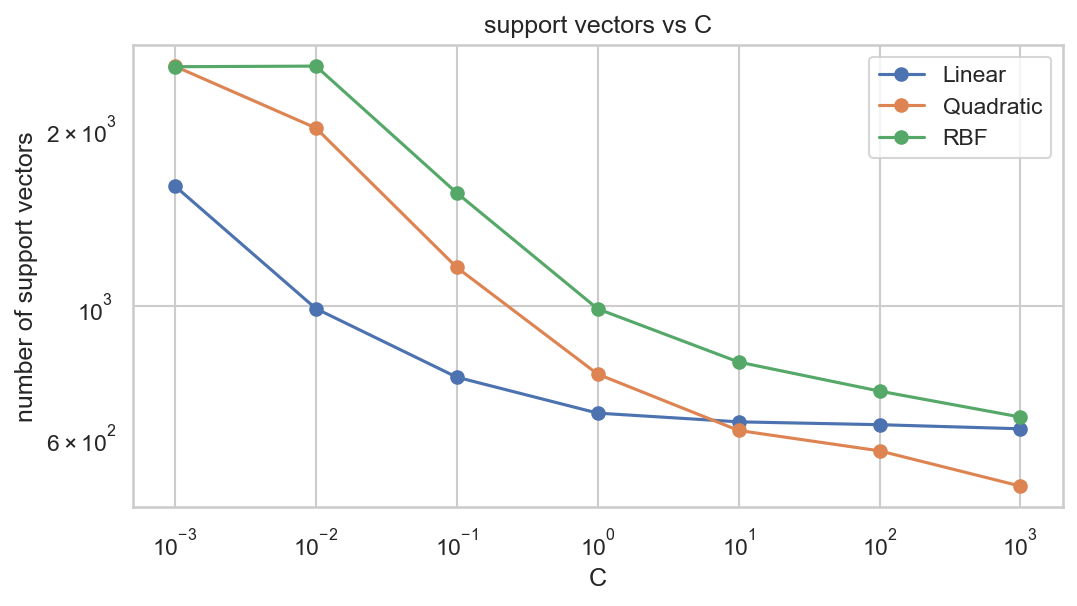
\includegraphics[width=0.55\linewidth]{figures/support_vectors.png}
\caption{Number of support vectors vs.\ $C$.}
\end{figure}

\subsection*{Extra: a log transform of the features}
The frequency and capital-run features are extremely right-skewed. After standardisation a handful of huge values still dominate the kernel
distances. Applying $\log(1+x)$ before standardising, and re-tuning $C$ for each kernel, improves every kernel:
\begin{table}[H]\centering
\begin{tabular}{lcccc}\toprule
Kernel & Standardised: test acc.\ (best $C$) & log + standardised: best $C$ & train acc. & test acc.\\\midrule
Linear & 0.9356 (100) & 0.1 & 0.9422 & 0.9479\\
Quadratic & 0.9392 (1) & 1 & 0.9562 & 0.9500\\
RBF & 0.9392 (10) & 10 & 0.9832 & \textbf{0.9551}\\\bottomrule
\end{tabular}
\end{table}
With the log transform the RBF kernel becomes clearly the best (95.5\%, +1.6 points), and the linear kernel needs only $C=0.1$ instead of 100. Once the
heavy tails are compressed, the classes are easier to separate, and the RBF kernel's notion of distance becomes meaningful across all features rather
than being driven by the few emails with very long runs of capitals. For an SVM on Spambase, how the features are preprocessed matters as much as the choice of kernel.

\end{document}
